\documentclass[11pt,a4paper]{article}

\usepackage{../../templates/style}

\begin{document}

\begin{problem}{ล้อมกรอบ (border)}{standard input}{standard output}{1 second}{16 megabytes}

    กำหนดตารางขนาด $N \times N$ $(1 \leq N \leq 100)$ โดยที่ขอบของตารางแต่ละขอบมีเลขเขียนกำกับเอาไว้ เช่น

\begin{figure}[h!]
\centering
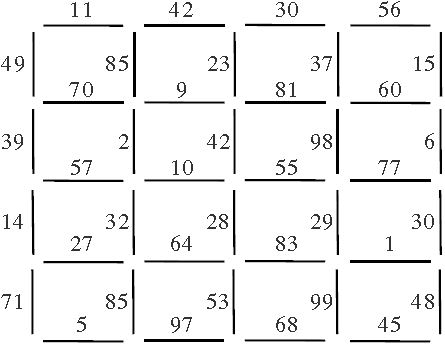
\includegraphics[width=0.45\textwidth]{../latex/img/1068/1068-1.png}
\end{figure}



    เราต้องการล้อมกรอบพื้นที่จำนวน $K$ $(1 \leq K \leq N^2)$ ช่อง เช่นถ้า $K = 5$ วิธีหนึ่ง ที่อาจจะล้อมกรอบพื้นที่เป็นดังต่อไปนี้
 
\begin{figure}[h!]
\centering
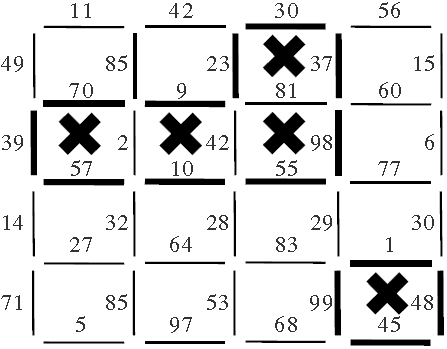
\includegraphics[width=0.45\textwidth]{../latex/img/1068/1068-2.png}
\end{figure}



    การล้อมกรอบต้องเสียค่าใช้จ่าย ซึ่ง เราสามารถคำนวณค่าใช้จ่ายได้ตามขั้นตอนต่อไปนี้
 
\begin{enumerate}

\item จำแนกขอบที่ล้อมกรอบบริเวณ $K$ ช่องดังกล่าว (ขอบเส้นหนาในรูปข้างบน) ออกเป็นสี่ชนิด ได้แก่
\begin{itemize}
\item ขอบบน คือ ขอบแนวนอนที่อยู่บนสุดของตาราง หรือช่องที่อยู่ใต้มันเป็นช่องที่ถูกล้อมกรอบ และช่องที่อยู่เหนือมันเป็นช่องที่ไม่ถูกล้อมกรอบ ในตัวอย่างคือขอบที่มีหมายเลข 70, 9, 30, และ 1

\item ขอบล่าง คือ ขอบแนวนอนที่อยู่ล่างสุดของตาราง หรือช่องที่อยู่เหนือมันเป็นช่องที่ถูกล้อมกรอบ และช่องที่อยู่ใต้มันเป็นช่องที่ไม่ถูกล้อมกรอบ ในตัวอย่างคือขอบที่มีหมายเลข 57, 10, 55, และ 45

\item ขอบซ้าย คือ ขอบแนวตั้ง ที่อยู่ซ้ายสุดของตาราง หรือช่องที่อยู่ด้านขวาของมันเป็นช่องที่ถูกล้อมกรอบ และช่องที่อยู่ด้านซ้ายของมันเป็นช่องที่ไม่ถูกล้อมกรอบ ในตัวอย่างคือขอบที่มีหมายเลข 23, 39, และ 99

\item ขอบขวา คือ ขอบแนวตั้ง ที่อยู่ขวาสุดของตาราง หรือช่องที่ทางด้านซ้ายของมันเป็นช่องที่ถูกล้อมกรอบ และช่องที่อยู่ด้านขวาของมันเป็นช่องที่ไม่ถูกล้อมกรอบ ในตัวอย่างคือ ขอบที่มีหมายเลข 37, 98, และ 48
\end{itemize}  
\item ทำการคำนวณค่าใช้จ่ายโดยใช้สูตรต่อไปนี้:\\ค่าใช้จ่าย$= 3\times$ผลรวมเลขขอบบน$+ 5 \times$ผลรวมเลขขอบซ้าย$- 3 \times$ผลรวมเลขขอบล่าง$- 5 \times$ผลรวมเลขขอบขวา
 \end{enumerate}
 
    ดังนั้นค่าใช้จ่ายในการล้อมกรอบดังรูปข้างบนจึงมีค่าเท่ากับ
 $$3 \times (70+9+23+30+1) + 5 \times (23+39+99) - 3\times (57+10+55+45) - 5\times (37+98+48) = -212$$
     เราอาจจะล้อมพื้นที่ $5$ ช่องได้อีกหนึ่งวิธี คือ

\begin{figure}[h!]
\centering
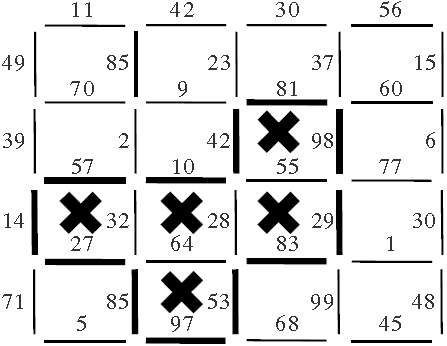
\includegraphics[width=0.45\textwidth]{../latex/img/1068/1068-3.png}
\end{figure}


    โดยในกรณีนี้ค่าใช้จ่ายในการล้อมกรอบจะมีค่าเท่ากับ
$3\times (57+10+81) + 5\times (42+14+85) - 3\times (27+97+83) - 5\times(98+29+53) = -372$

\bigskip
\underline{\textbf{โจทย์}}  จงเขียนโปรแกรมรับค่า $N$ และ $K$ พร้อมทั้งหมายเลขบนขอบทั้งหมดของตาราง แล้วคำนวณค่าใช้จ่ายที่น้อยที่สุดเท่าที่จะเป็นไปได้ในการล้อมกรอบพื้นที่ $K$ ช่อง

\InputFile

\textbf{บรรทัดแรก} มีจำนวนเต็มบวก $N$ และ $K$ ซึ่งมีขอบเขตดังที่ได้กล่าวไปแล้วข้างต้น

\textbf{บรรทัดที่ $2$ ถึง $2N+2$} เป็นข้อมูลหมายเลขที่อยู่บนขอบ เรียงจากเหนือลงใต้และซ้ายไปขวา กล่าวคือ
\newpage

\begin{itemize}
   
\item \textbf{ในบรรทัดที่ $i+1$ เมื่อ $i$ เป็นเลขคู่} จะมีตัวเลขอยู่ $N$ ตัว แสดงหมายเลขของขอบแนวนอนเรียงจากซ้ายไปขวา
   
\item \textbf{ในบรรทัดที่ $i+1$ เมื่อ $i$ เป็นเลขคี่} จะมีตัวเลขอยู่ $N+1$ ตัว แสดงหมายเลขของขอบแนวตั้งเรียงจากซ้ายไปขวา
    \end{itemize}
หมายเลขบนขอบแต่ละหมายเลขเป็นจำนวนเต็มที่ไม่เป็นลบที่มีค่าไม่เกิน $10\,000$

\OutputFile

\textbf{มีบรรทัดเดียว} พิมพ์ค่าใช้จ่ายที่น้อยที่สุดที่เป็นไปได้ในการล้อมกรอบพื้นที่ $K$ ช่อง

\Examples

\begin{example}
\exmp{4 5
11 42 30 56
49 85 23 37 15
70 9 81 60
39 2 42 98 6
57 10 55 77
14 32 28 29 30
27 64 83 1
71 85 53 99 48
5 97 68 45}{-1170}%
\end{example}


\Source

การแข่งขัน YTOPC กุมภาพันธ์ 2552

\end{problem}

\end{document}